\RequirePackage{luatex85}

% for notes environment
\usepackage{xsavebox}
\usepackage{hyperref}
\usepackage{graphicx}
\usepackage{luatexja}
\usepackage[hiragino-pro,deluxe,nfssonly,jis2004]{luatexja-preset}
\usepackage{fontspec}
\usepackage{epigraph}
\usepackage{etoolbox}
\usepackage{tikz}
\usepackage{framed}
\usepackage{mathtools}
\usepackage{listings}
\usepackage{libertine}
\usepackage[libertine]{newtxmath}
\usepackage{bxcoloremoji}
\usepackage{xcolor}
\usepackage{diagbox}
\usepackage{caption}
\usepackage{appendixnumberbeamer}
\usepackage{multirow}
\usepackage{xpatch}
\usepackage{multicol}
\usepackage{tabularx}
\usepackage{amsmath}
\usepackage{amsthm}
\usepackage{blochsphere}
\usepackage{bxtexlogo}
\usepackage[braket, qm]{qcircuit}
\bxtexlogoimport{SATySFi}

\usetikzlibrary{fit}

\setmonofont{CMU Typewriter Text}

\definecolor{links}{HTML}{2A1B81}
\hypersetup{colorlinks,linkcolor=,urlcolor=links}

\usetheme{Boadilla}
\usecolortheme{seahorse}
% \usefonttheme{serif}


\xpatchcmd{\itemize}
  {\def\makelabel}
  {\ifnum\@itemdepth=1\relax
     \setlength\itemsep{1.2ex}% separation for first level
   \else
     \ifnum\@itemdepth=2\relax
       \setlength\itemsep{0.8ex}% separation for second level
       \setlength\topsep{1.2ex}
     \else
       \ifnum\@itemdepth=3\relax
         \setlength\itemsep{0.05ex}% separation for third level
         \setlength\topsep{0.8ex}
   \fi\fi\fi\def\makelabel
  }
 {}
 {}

\setbeamercolor{page number in head/foot}{bg=blue!10}
\setbeamertemplate{footline}{%
  \leavevmode%
  \hbox{%
    \begin{beamercolorbox}[wd=.3\paperwidth,ht=2.25ex,dp=1ex,center]{author in head/foot}%
      \usebeamerfont{author in head/foot}\insertshortauthor\hspace*{1ex}(\insertshortinstitute)
    \end{beamercolorbox}%
    \begin{beamercolorbox}[wd=.2\paperwidth,ht=2.25ex,dp=1ex,center]{title in head/foot}%
      \usebeamerfont{title in head/foot}\insertshorttitle
    \end{beamercolorbox}%
    \begin{beamercolorbox}[wd=.4\paperwidth,ht=2.25ex,dp=1ex,center]{date in head/foot}%
      \insertshortdate{} @ \InsertConference
    \end{beamercolorbox}%
    \begin{beamercolorbox}[wd=.1\paperwidth,ht=2.25ex,dp=1ex,center]{page number in head/foot}%
      \insertframenumber{} / \inserttotalframenumber\hspace*{1ex}
    \end{beamercolorbox}}%
  \vskip0pt%
}

\beamertemplatenavigationsymbolsempty

\setbeamertemplate{bibliography item}{\insertbiblabel}
\setbeamersize{description width=1cm}
\setbeamertemplate{items}[circle]
\setbeamertemplate{section in toc}[circle]
\setbeamertemplate{subsection in toc}{%
  \leavevmode\leftskip=2em
  {%
    \usebeamerfont*{itemize item}%
    \usebeamercolor{subsection number projected}%
    \color{bg}%
    \raise1.25pt\hbox{\donotcoloroutermaths$\bullet$}}%
  \hskip1.5ex\inserttocsubsection\par}

% Definitions for the title page
\newcommand*{\GitHub}[1]{%
  \gdef\InsertGitHub{#1}%
}
\newcommand*{\Email}[1]{%
  \gdef\InsertEmail{\href{mailto:#1}{#1}}%
}
\newcommand*{\Conference}[1]{%
  \gdef\InsertConference{#1}%
}
\setbeamerfont{title}{size=\huge, series=\bfseries, family=\mcfamily\rmfamily}
\setbeamercolor{title}{bg=white}
\setbeamerfont{subtitle}{size=\small, series=\mdseries, family=\mcfamily\rmfamily}%\gtfamily\sffamily}
\setbeamerfont{email}{size=\scriptsize, family=\ttfamily}
\setbeamercolor{email}{bg=white}
\setbeamerfont{date}{shape=\itshape, family=\rmfamily}
\setbeamerfont{vc}{size=\scriptsize, family=\ttfamily}
\setbeamercolor{vc}{bg=white}

\renewcommand{\figurename}{Fig}

\input{vc.tex}

\setbeamertemplate{title page}
{%
  \vbox{}
  \vfill
  \begingroup
    \centering
    \hrulefill\par%
    \vskip1ex\par%
    \begin{beamercolorbox}[sep=0pt,center,shadow=false,rounded=true]{title}
      \vfill
      \usebeamerfont{title}\inserttitle\par%
      \ifx\insertsubtitle\@empty%
      \else%
        \vskip0.5ex%
        {\usebeamerfont{subtitle}\usebeamercolor[fg]{subtitle}\insertsubtitle\par}%
      \fi%
      \vfill  
    \end{beamercolorbox}%
    \hrulefill\par%
    \vskip2ex%
    \begin{beamercolorbox}[sep=0pt,center,shadow=false,rounded=true]{author}
      \usebeamerfont{author}\insertauthor
    \end{beamercolorbox}
    \begin{beamercolorbox}[sep=0pt,center,shadow=false,rounded=true]{email}
      \usebeamerfont{email}\InsertEmail
    \end{beamercolorbox}
    \vskip0.1ex
    \begin{beamercolorbox}[sep=5pt,center,shadow=false,rounded=true]{institute}
      \usebeamerfont{institute}\insertinstitute
    \end{beamercolorbox}
    \begin{beamercolorbox}[sep=5pt,center,shadow=false,rounded=true]{date}
      \usebeamerfont{date}\insertdate \normalfont @ \InsertConference
    \end{beamercolorbox}
    \begin{beamercolorbox}[sep=0pt,center,shadow=false,rounded=true]{vc}
      \usebeamerfont{vc}
      \url{https://github.com/\InsertGitHub} (\texttt{\GITAbrHash})
    \end{beamercolorbox}
    % {\centering
    %   \href{https://creativecommons.org/licenses/by-nc/4.0/}{%
    %     \includegraphics[width=0.1\textwidth]{img/by-nc.pdf}%
    %   }%
    % }
    {\usebeamercolor[fg]{titlegraphic}\inserttitlegraphic\par}
  \endgroup
  \vfill
}
\setbeamertemplate{blocks}[rounded][shadow=false]

% ============ ここを消すとNote消える ================
% \mode<handout>{%
%   \usepackage{pgfpages}
%   \setbeameroption{show notes on second screen=right}
%   \setbeamertemplate{note page}{%
%     \vspace{2ex}\insertnote%
%   }
% }
% ============ ここを消すとNote消える ================


\renewcommand{\kanjifamilydefault}{\gtdefault}

\setbeamertemplate{caption}[numbered]
\resetcounteronoverlays{lstlisting}
\definecolor{bluegray}{rgb}{0.4, 0.6, 0.8}
\DeclareCaptionFormat{listing}{{\color{bluegray}\lstlistingname}#2#3}
\captionsetup[lstlisting]{format=listing, font={footnotesize}}
\captionsetup[figure]{name={図}}
\captionsetup[table]{name={表}}
\setbeamerfont{footnote}{size=\scriptsize}

\setmonofont[Ligatures=TeX]{CMU Typewriter Text}

\setbeamertemplate{items}[circle]

\newfontfamily\quotefont[Ligatures=TeX]{Linux Libertine O} % selects Libertine as the quote font

\newcommand*\quotesize{60} % if quote size changes, need a way to make shifts relative
% Make commands for the quotes
\newcommand*{\openquote}{%
  \tikz[remember picture,overlay,xshift=0em,yshift=-3ex]
  \node (OQ) {\quotefont\fontsize{\quotesize}{\quotesize}\selectfont``};\kern0pt%
  \par\quad\par
}

\newcommand*{\closequote}[1]
  {\tikz[remember picture,overlay,xshift=1ex,yshift={#1}]
   \node (CQ) {\quotefont\fontsize{\quotesize}{\quotesize}\selectfont''};}

\newcommand*\shadedauthorformat{\emph} % define format for the author argument

% Now a command to allow left, right and centre alignment of the author
\newcommand*\authoralign[1]{%
  \if#1l
    \def\authorfill{}\def\quotefill{\hfill}
  \else
    \if#1r
      \def\authorfill{\hfill}\def\quotefill{}
    \else
      \if#1c
        \gdef\authorfill{\hfill}\def\quotefill{\hfill}
      \else\typeout{Invalid option}
      \fi
    \fi
  \fi}
% wrap everything in its own environment which takes one argument (author) and one optional argument
% specifying the alignment [l, r or c]
%
\newenvironment{shadequote}[2][l]%
{\hspace{0.5ex}
\authoralign{#1}
\ifblank{#2}
   {\def\shadequoteauthor{}\def\yshift{-1ex}\def\quotefill{\hfill}}
   {\def\shadequoteauthor{\par\authorfill\shadedauthorformat{#2}}\def\yshift{3ex}}
\begin{quote}\normalfont\openquote}
{\shadequoteauthor\quotefill\closequote{\yshift}\end{quote}}

\makeatletter
\def\@fnsymbol#1{\ensuremath{\ifcase#1\or \dagger\or \ddagger\or
   \mathsection\or \mathparagraph\or \|\or **\or \dagger\dagger
   \or \ddagger\ddagger \else\@ctrerr\fi}}
\makeatother

\renewcommand{\thefootnote}{\fnsymbol{footnote}}
\renewcommand{\thempfootnote}{\fnsymbol{mpfootnote}}
\newcommand\ballcircle[1]{%
  {%
    \usebeamercolor{enumerate item}%
    \tikzset{beameritem/.style={circle,inner sep=0,minimum size=2ex,text=enumerate item.bg,fill=enumerate item.fg}}%
    \tikz[baseline=(n.base)]\node(n)[beameritem]{\sffamily#1};%
  }%
}
\newcommand\ballref[1]{%
  \ballcircle{\ref{#1}}%
}

\usetikzlibrary{calc}
\usetikzlibrary{shapes.callouts} 

\pgfkeys{%
    /calloutquote/.cd,
    width/.code                   = {\def\calloutquotewidth{#1}},
    position/.code                = {\def\calloutquotepos{#1}}, 
    author/.code                  = {\def\calloutquoteauthor{#1}},
    at/.code                      = {\def\calloutquoteat{#1}},
    sign/.code                    = {\def\calloutquotesign{#1}},
    /calloutquote/.unknown/.code  = {\let\searchname=\pgfkeyscurrentname
                                      \pgfkeysalso{\searchname/.try=#1,                        
                                      /tikz/\searchname/.retry=#1},\pgfkeysalso{\searchname/.try=#1,
                                      /pgf/\searchname/.retry=#1}
                                    }
}

\makeatletter

\newsavebox\temp@simple@callout@author@box
\newcommand\calloutquote[2][]{%
  \pgfkeys{/calloutquote/.cd,
    width    = 5cm,
    position = {(0.5,-0.2)},
    at       = {(0,0)},
    author   = {},
    sign     = {+}
  }%
  \pgfqkeys{/calloutquote}{#1}%
  \sbox{\temp@simple@callout@author@box}{\mbox{%
    \begin{tabular}{l}
      \calloutquoteauthor%
    \end{tabular}
  }}%
  \node[thin, draw=black!50, rectangle callout,callout relative pointer={\calloutquotepos},align=center,text width=\calloutquotewidth,/calloutquote/.cd,
     #1] (tmpcall) at \calloutquoteat {#2};
  \node at ($ (tmpcall.pointer) - (-\calloutquotesign0.5\wd\temp@simple@callout@author@box,0.7\ht\temp@simple@callout@author@box) $) {\calloutquoteauthor};
}

\newsavebox\temp@simple@callout@box
\newcommand{\simplecallout}[4][{}]{%
  \sbox{\temp@simple@callout@box}{\mbox{%
    \begin{tabular}{l}
      #4%
    \end{tabular}
  }}%
  \begin{center}%
    \begin{tikzpicture}%
      \calloutquote[width=1.05\wd\temp@simple@callout@box,position={(#2.5,-0.2)},fill=#3,rounded corners,author={#1},sign=#2]{
        #4%
      }%
    \end{tikzpicture}%
  \end{center}
}

\makeatother
\newfontfamily{\listingfont}[Scale=0.85]{Menlo}
\definecolor{dkgreen}{rgb}{0,0.6,0}
\definecolor{gray}{rgb}{0.5,0.5,0.5}
\definecolor{mauve}{rgb}{0.58,0,0.82}

\makeatletter
\lst@CCPutMacro\lst@ProcessOther {"2D}{\lst@ttfamily{-{}}{-{}}}
\@empty\z@\@empty
\makeatother

\lstdefinestyle{csharp}{
  numbers=left,
  language=[Sharp]C
}

\lstdefinestyle{cil}{
  numbers=left,
  language=CIL
}

\lstdefinestyle{plain}{
  basicstyle=\listingfont\scriptsize,
  language=Plain,
  showstringspaces=false,
  showtabs=false,
  stringstyle=\listingfont\scriptsize\color{mauve},
  tabsize=2
}

\lstdefinestyle{sh}{
  numbers=left,
  language=sh
}

\lstdefinestyle{c}{
  numbers=left,
  language=C
}

\lstdefinestyle{python}{
  numbers=left,
  language=Python
}

\lstdefinestyle{asm-x86}{
  numbers=left
}

\lstdefinestyle{pseudo-code}{
  numbers=left,
  keywords=[6]{for,from,to,endfor,while,endwhile}
}

\lstdefinestyle{bitcoin-script}{
  mathescape=true
}

\lstset{
  basicstyle=\listingfont,
  frame=single,
  xleftmargin=2em,
  xrightmargin=1em,
  breaklines=true
}

\lstdefinestyle{scala}{
  basicstyle=\listingfont\scriptsize,
  breakatwhitespace=false,
  language=scala,
  captionpos=b,
  commentstyle=\listingfont\scriptsize\color{dkgreen},
  extendedchars=true,
  xleftmargin=1em,
  xrightmargin=1em,
  keepspaces=true,
  keywordstyle=\listingfont\scriptsize\color{blue},
  emphstyle=\listingfont\scriptsize\color{cyan},
  rulecolor=\listingfont\scriptsize\color{black},
  showspaces=false,
  showstringspaces=false,
  showtabs=false,
  stringstyle=\listingfont\scriptsize\color{mauve},
  tabsize=2
}

\lstdefinestyle{go}{
  basicstyle=\listingfont\scriptsize,
  breakatwhitespace=false,
  language=go,
  captionpos=b,
  commentstyle=\listingfont\scriptsize\color{dkgreen},
  extendedchars=true,
  xleftmargin=1em,
  xrightmargin=1em,
  keepspaces=true,
  keywordstyle=\listingfont\scriptsize\color{blue},
  emphstyle=\listingfont\scriptsize\color{cyan},
  rulecolor=\listingfont\scriptsize\color{black},
  showspaces=false,
  showstringspaces=false,
  showtabs=false,
  stringstyle=\listingfont\scriptsize\color{mauve},
  tabsize=2
}

\lstdefinestyle{js}{
  basicstyle=\listingfont\scriptsize,
  breakatwhitespace=false,
  language=JavaScript,
  captionpos=b,
  commentstyle=\listingfont\scriptsize\color{dkgreen},
  extendedchars=true,
  xleftmargin=1em,
  xrightmargin=1em,
  keepspaces=true,
  keywordstyle=\listingfont\scriptsize\color{blue},
  emphstyle=\listingfont\scriptsize\color{cyan},
  rulecolor=\listingfont\scriptsize\color{black},
  showspaces=false,
  showstringspaces=false,
  showtabs=false,
  stringstyle=\listingfont\scriptsize\color{mauve},
  tabsize=2
}

\lstdefinestyle{css}{
  basicstyle=\listingfont\scriptsize,
  breakatwhitespace=false,
  language=CSS,
  captionpos=b,
  commentstyle=\listingfont\scriptsize\color{dkgreen},
  extendedchars=true,
  xleftmargin=1em,
  xrightmargin=1em,
  keepspaces=true,
  keywordstyle=\listingfont\scriptsize\color{blue},
  emphstyle=\listingfont\scriptsize\color{cyan},
  rulecolor=\listingfont\scriptsize\color{black},
  showspaces=false,
  showstringspaces=false,
  showtabs=false,
  stringstyle=\listingfont\scriptsize\color{mauve},
  tabsize=2
}

\lstdefinestyle{html}{
  basicstyle=\listingfont\scriptsize,
  breakatwhitespace=false,
  language=HTML5,
  captionpos=b,
  commentstyle=\listingfont\scriptsize\color{dkgreen},
  extendedchars=true,
  xleftmargin=1em,
  xrightmargin=1em,
  keepspaces=true,
  keywordstyle=\listingfont\scriptsize\color{blue},
  emphstyle=\listingfont\scriptsize\color{cyan},
  rulecolor=\listingfont\scriptsize\color{black},
  showspaces=false,
  showstringspaces=false,
  showtabs=false,
  stringstyle=\listingfont\scriptsize\color{mauve},
  tabsize=2
}

\lstdefinelanguage{Plain}{
  morestring=[b]",
  morestring=[b]'
}

\lstdefinelanguage{scala}{
  morekeywords={abstract,case,catch,class,def,%
    do,else,extends,false,final,finally,%
    for,if,implicit,import,match,mixin,%
    new,null,object,override,package,%
    private,protected,requires,return,sealed,%
    super,this,throw,trait,true,try,%
    type,val,var,while,with,yield},
  moreemph={Byte,Short,Int,Long,Float,Double,Char,
    String,Boolean,Unit,Null,Nothing,Any,AnyRef,
    Left,Right,Either},
  otherkeywords={=>,<-,<\%,<:,>:,\#,@},
  sensitive=true,
  morecomment=[l]{//},
  morecomment=[n]{/*}{*/},
  morestring=[b]",
  morestring=[b]',
  morestring=[b]"""
}

\lstdefinelanguage{golang}%
  {morekeywords=[1]{package,import,func,type,struct,return,defer,panic,%
     recover,select,var,const,iota},%
   morekeywords=[2]{string,uint,uint8,uint16,uint32,uint64,int,int8,int16,%
     int32,int64,bool,float32,float64,complex64,complex128,byte,rune,uintptr,%
     error,interface},%
   morekeywords=[3]{map,slice,make,new,nil,len,cap,copy,close,true,false,%
     delete,append,real,imag,complex,chan,},%
   morekeywords=[4]{for,break,continue,range,go,goto,switch,case,fallthrough,if,%
     else,default,},%
   morekeywords=[5]{Println,Printf,Error,Print,},%
   sensitive=true,%
   morecomment=[l]{//},%
   morecomment=[s]{/*}{*/},%
   morestring=[b]',%
   morestring=[b]",%
   morestring=[s]{`}{`},%
}

\lstdefinelanguage{JavaScript}{%
  keywords={typeof, new, true, false, catch, function, return, null, catch, switch, var, if, in, while, do, else, case, break},
  keywordstyle=\color{blue}\bfseries,
  ndkeywords={class, export, boolean, throw, implements, import, this},
  ndkeywordstyle=\color{darkgray}\bfseries,
  identifierstyle=\color{black},
  sensitive=false,
  comment=[l]{//},
  morecomment=[s]{/*}{*/},
  commentstyle=\color{purple}\ttfamily,
  stringstyle=\color{red}\ttfamily,
  morestring=[b]',
  morestring=[b]"
}

\lstdefinelanguage{CSS}{
  keywords={url},
  morekeywords={@import},
  keywordstyle=\color{blue},
  morecomment=[s]{/*}{*/}
}

\lstdefinelanguage{HTML5}{
    sensitive=true,
    keywords={%
    % JavaScript
    typeof, new, true, false, catch, function, return, null, catch, switch, var, if, in, while, do, else, case, break,
    % HTML
    html, title, meta, style, head, body, script, canvas,
    % CSS
    border:, transform:, -moz-transform:, transition-duration:, transition-property:,
    transition-timing-function:
    },
    % http://texblog.org/tag/otherkeywords/
    otherkeywords={<, >, \/},   
    ndkeywords={class, export, boolean, throw, implements, import, this},   
    comment=[l]{//},
    % morecomment=[s][keywordstyle]{<}{>},  
    morecomment=[s]{/*}{*/},
    morecomment=[s]{<!}{>},
    morestring=[b]',
    morestring=[b]",    
    alsoletter={-},
    alsodigit={:}
}
\newenvironment{notes}
  {%
    \begin{xlrbox}{NotesBox}
    \begin{minipage}{.95\textwidth}
    \small\rmfamily\mcfamily
    \begin{itemize}
    \setlength{\itemindent}{0em}
    \setlength{\footnotesep}{5mm}
  }{%
    \end{itemize}
    \end{minipage}
    \end{xlrbox}
    \note{\theNotesBox}}

\def\AtSOne#1\csod{%
	\begin{array}{c|}
		\hline
		#1\\
		\hline
	\end{array}
}%
\def\AtSTwo#1,#2\csod{%
	\begin{array}{c|c|}
		\hline
		#1 & #2\\
		\hline
	\end{array}
}%
\def\AtSThree#1,#2,#3\csod{%
	\begin{array}{c|c|c|}
		\hline
		#1 & #2 & #3\\
		\hline
	\end{array}
}%
\def\AtSFour#1,#2,#3,#4\csod{%
	\begin{array}{c|c|c|c|}
		\hline
		#1 & #2 & #3 & #4\\
		\hline
	\end{array}
}%
\def\AtSFive#1,#2,#3,#4,#5\csod{%
	\begin{array}{c|c|c|c|c|}
		\hline
		#1 & #2 & #3 & #4 & #5\\
		\hline
	\end{array}
}%
\def\AtSSix#1,#2,#3,#4,#5,#6\csod{%
	\begin{array}{c|c|c|c|c|c|}
		\hline
		#1 & #2 & #3 & #4 & #5 & #6\\
		\hline
	\end{array}
}
\newcommand{\SOne}[1]{\AtSOne#1\csod}
\newcommand{\STwo}[1]{\AtSTwo#1\csod}
\newcommand{\SThree}[1]{\AtSThree#1\csod}
\newcommand{\SFour}[1]{\AtSFour#1\csod}
\newcommand{\SFive}[1]{\AtSFive#1\csod}
\newcommand{\SSix}[1]{\AtSSix#1\csod}
\newcommand\card[2]{%
  \setlength{\fboxsep}{0pt}%
  \fcolorbox{black}{#1}{%
    \hphantom{\rule{0.05em}{0ex}}%
    #2%
    \hphantom{\rule{0.05em}{0ex}}%
    \vphantom{\rule[-0.5ex]{0em}{2.5ex}}%
  }%
}%
\definecolor{coolblack}{rgb}{0.0, 0.18, 0.39}
\newcommand\heartcard{\card{white}{\color{red}{♥}}}
\newcommand\clubcard{\card{white}{\color{coolblack}{♣}}}
\newcommand\commitedcard{\card{gray!20}{\hphantom{\rule{0.28em}{0ex}}?\hphantom{\rule{0.28em}{0ex}}}}%}}
% \def\yescards{\heartcard\,\heartcard\,\clubcard}
% \def\nocards{\heartcard\,\clubcard\,\clubcard}
% \def\threecommitedcards{\commitedcard\,\commitedcard\,\commitedcard}
% \def\threeheartcards{\heartcard\,\heartcard\,\heartcard}
% \def\threeclubcards{\clubcard\,\clubcard\,\clubcard}

\newcommand\ce[1]{%
  \coloremojiucs{#1}
}

\newcommand*{\lstitem}[1]{
  \setbox0\hbox{\lstinline{#1}}
  \item[\usebox0]
}

\presetkeys{todonotes}{inline, noinlinepar}{}

\renewcommand{\arraystretch}{1.2}
\newcolumntype{Y}{>{\centering\arraybackslash}X}

\title[Quantum Covert Lottery]{%
  Quantum Covert Lottery
}
\subtitle{高速化ではない量子コンピュータの応用}
\author[吉村 優]{%
  吉村 優(\textsc{Yoshimura} Hikaru)
}
\Email{hikaru\_yoshimura@r.recruit.co.jp}
\date[October 7-9, 2023]{%
  \oldstylenums{October 7-9, 2023}
}
\Conference{第56回 情報科学若手の会}
\institute[\InsertEmail]{%
  株式会社リクルート(Recruit Co., Ltd) \\
  
\includegraphics[width=3cm]{./img/6_Brandlogo_2_Color.jpg}
}
\GitHub{y-yu/quantum-covert-lottery-slide}

\newcommand{\facesize}{1cm}
\newcommand\alicecallout[2]{
  \simplecallout[{
\includegraphics[width=\facesize]{./img/alice_face.png}}]{#1}{cyan!10}{#2}
}
\newcommand\bobcallout[2]{
  \simplecallout[{
\includegraphics[width=\facesize]{./img/bob_face.png}}]{#1}{orange!10}{#2}
}


\newcommand{\Zero}{\left(
    \begin{array}{c}
      1 \\
      0
    \end{array}
  \right)}

\newcommand{\One}{\left(
    \begin{array}{c}
      0 \\
      1
    \end{array}
  \right)}

\newcommand{\天国}{\textcolor{cyan}{\ket{\text{天国}}}}
\newcommand{\地獄}{\textcolor{cyan}{\ket{\text{地獄}}}}
\newcommand{\生}{\textcolor{orange}{\ket{\text{生}}}}
\newcommand{\死}{\textcolor{orange}{\ket{\text{死}}}}

\begin{document}

\frame{\maketitle}

\begin{frame}
  \frametitle{自己紹介}
  
  \begin{columns}
    \begin{column}{0.3\textwidth}
      \begin{center}
        \begin{figure}
          
\includegraphics[width=0.95\textwidth]{img/bird2x.png}
        \end{figure}
      \end{center}
 
      \begin{table}[h]
        \begin{tabular}{ll}
          Twitter & \href{https://twitter.com/\_yyu\_}{@\_yyu\_} \\
          GitHub &  \href{https://github.com/y-yu}{y-yu} \\
        \end{tabular}
      \end{table}
    \end{column}
    \begin{column}{0.7\textwidth}
      \begin{itemize}
        \item 筑波大学 情報学群 情報科学類卒(2011-15,学士)
        \begin{itemize}
          \item プログラム論理研究室で型システムの研究
        \end{itemize}

        \item スタディサプリENGLISH バックエンド(Scala)

        \item 未踏ターゲット2018(ゲート式量子コンピュータ)

        \item CTF(\url{https://urandom.team/})
        \begin{itemize}
          \item SECCON CTF 2023 Quals 72位(国内26位)
        \end{itemize}

        \item iOS・macOS向けコーヒー抽出支援アプリ\ce{:coffee:}

        \item プログラミング
        \begin{itemize}
          \item Scala, \LaTeX, Rust, Swift
          \item \SATySFi のバージョン\texttt{0.1.0}待ってます!\ce{:pray:}
        \end{itemize}
      \end{itemize}
    \end{column}
  \end{columns}
\end{frame}

\begin{frame}
  \frametitle{目次}

  \tableofcontents
\end{frame}

\section{Covert Lotteryとは?}

\begin{frame}
  \frametitle{Covert Lotteryとは?}

  \begin{itemize}
    \item \emph{Covert Lottery}は\cite{covert_lottery_2021}で提案された、ちょっと変わった抽選
  \end{itemize}

  \pause
  \begin{shadequote}[r]{}
    参加者2人が1bit(= $0$ or $1$)のいずれかの希望があるとき、
    \begin{enumerate}
      \item 二人の希望が一致していれば、それが採用される
      \item 衝突していたらランダムにする
    \end{enumerate}
  \end{shadequote}

  \pause
  \simplecallout[{\LARGE\ce{:thinking:}}]{+}{cyan!10}{{\LARGE いったい何に使えるのか?}}
\end{frame}

\begin{frame}
  \frametitle{%
    奢り・割り勘問題\footnote{%
      \cite{covert_lottery_2021}では将棋などの先攻・後攻を決める問題を例にしている。%
    }%
  }

  \begin{columns}
    \begin{column}{0.7\textwidth}
      \begin{figure}[h]
        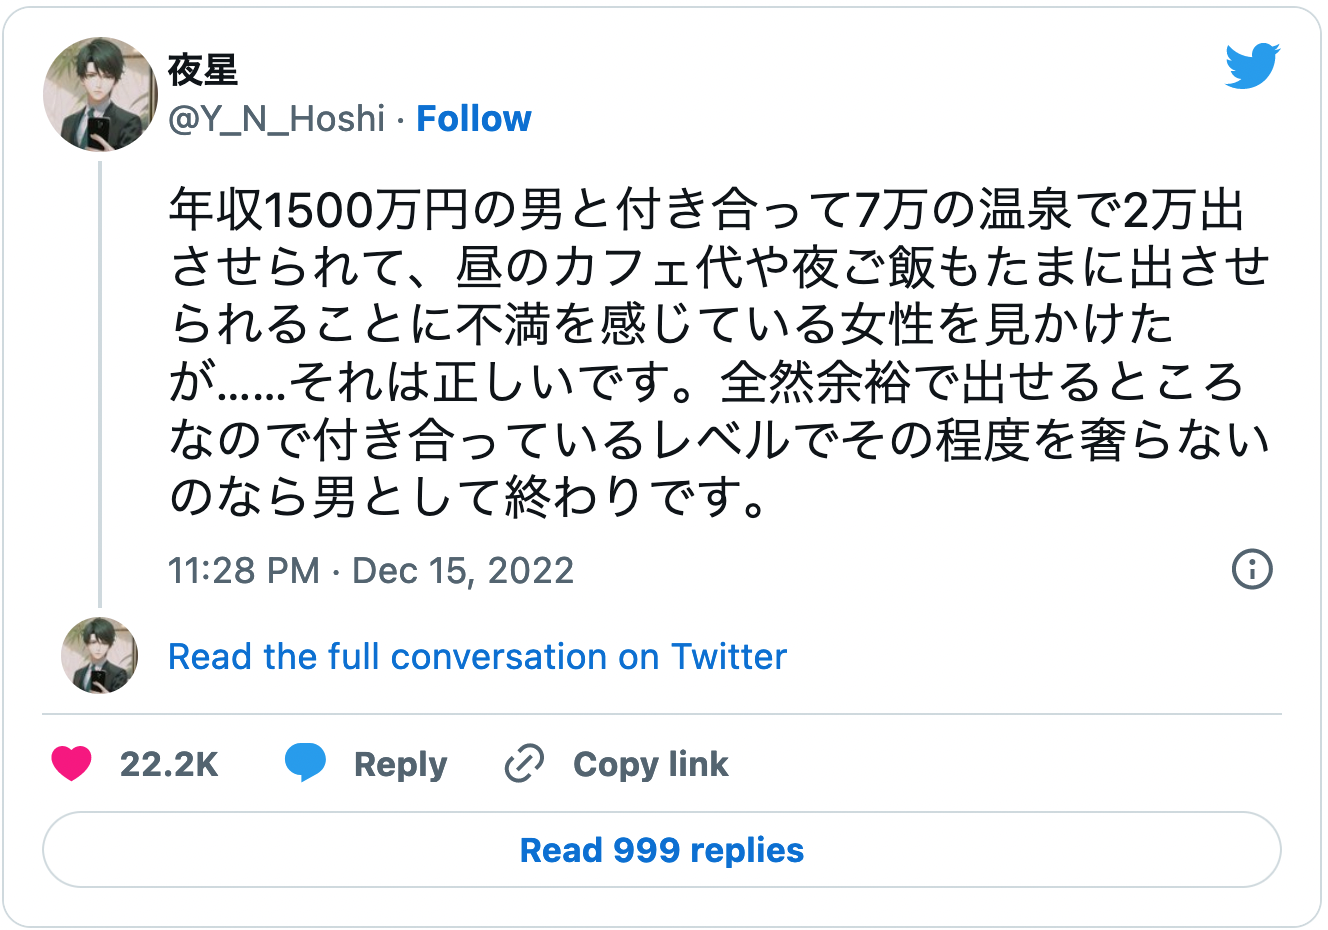
\includegraphics[width=0.85\textwidth]{./img/twitter.png}\cite{Y_N_Hoshi}
      \end{figure}
    \end{column}
    \begin{column}{0.3\textwidth}
      \pause
      \simplecallout[{\LARGE\ce{:sunglasses:}}]{+}{green!10}{{\large\ce{:point_left:}これか!?}}
    \end{column}
  \end{columns}
\end{frame}

\begin{frame}
  \frametitle{奢り・割り勘問題}

  \begin{shadequote}[r]{}
    アリスとボブの飲食費について下記のいずれにするか決定する問題
    \begin{enumerate}
      \item ボブが全額を奢る
      \item 割り勘とする
    \end{enumerate}
  \end{shadequote}

  \begin{columns}
    \begin{column}{0.5\textwidth}
      \centering
      \emph{アリス(Alice)}

      \begin{figure}[h]
        
\includegraphics[height=0.35\textheight]{img/alice.png}
      \end{figure}
    \end{column}
   
    \begin{column}{0.5\textwidth}
      \centering
      \emph{ボブ(Bob)}

      \begin{figure}[h]
        
\includegraphics[height=0.35\textheight]{img/bob.png}
      \end{figure}
    \end{column}
  \end{columns}
\end{frame}

\section{古典Covert Lotteryと情報リーク}

\begin{frame}
  \frametitle{%
    カードを用いた古典Covert Lottery\protect\footnote{%
      \cite{covert_lottery_2021}では3人以上への拡張も踏まえてやや複雑な方法が説明されており、
      このプロトコルは発表者が2人を前提に独自に簡略化したものとなっている。%
    }
  }
  次のように物理的なカード\footnote{%
    これらのカードはトランプのようにいずれも裏が\commitedcard となっており、
    裏向きになった状態でどちらのカードなのか特定することができない。%
  }を用いて行う

  \pause
  \begin{columns}
    \begin{column}{0.6\textwidth}
      \begin{enumerate}
        \item アリス・ボブに2枚のカード\heartcard,\clubcard を配る
        \item アリス・ボブは表\ref{tbl:card_meaning}に従って
        希望を裏向き\commitedcard にして提出する\label{enum:cards_commited}

        \item \ballref{enum:cards_commited}で提出されたカードをシャッフルする
        
        \item どちらか1枚をドローして表向きにする \label{enum:result}
      \end{enumerate}

      \ballref{enum:result}のカードを表\ref{tbl:card_meaning}に対応させてプロトコルの結果とする
    \end{column}
    \begin{column}{0.4\textwidth}
      \begin{table}[h]
        \caption{カードの意味}
        \label{tbl:card_meaning}
        \begin{tabularx}{0.9\textwidth}{@{}| Y | Y |@{}}
          \hline
          カード & 意味 \\ \hline
          \heartcard & ボブの奢り \\ \hline
          \clubcard & 割り勘 \\ \hline
        \end{tabularx}
      \end{table}
    \end{column}
  \end{columns}
\end{frame}

\begin{frame}
  \frametitle{ケーススタディ\ballcircle{1} --- 2人の希望が一致}

  \pause
  \begin{itemize}
    \item<+-> 2人の希望が一致しているので次のようなケース
      \begin{columns}
        \begin{column}{0.5\textwidth}
          \alicecallout{+}{\heartcard}
        \end{column}
        \begin{column}{0.5\textwidth}
          \bobcallout{-}{\heartcard}
        \end{column}
      \end{columns}

    \item<+-> これらをシャッフルして1枚選んだときは必ず\heartcard となる

    \item<+-> 2人の希望が一致していればこのように必ずそちらが選ばれる
  \end{itemize}
\end{frame}

\begin{frame}
  \frametitle{ケーススタディ\ballcircle{2} --- 2人の希望が衝突}

  \begin{itemize}
    \item<+-> 2人の希望が衝突しているので次のようなケース
      \begin{columns}
        \begin{column}{0.5\textwidth}
          \alicecallout{+}{\heartcard}
        \end{column}
        \begin{column}{0.5\textwidth}
          \bobcallout{-}{\clubcard}
        \end{column}
      \end{columns}

    \item<+-> これらをシャッフルしてランダムに選べば、結果は\heartcard,\clubcard それぞれ$\frac{1}{2}$の確率になる
    \begin{description}
      \item[結果が\heartcard]<+-> アリスの希望どおり
      \item[結果が\clubcard]<+-> ボブの希望どおり
    \end{description}
    \uncover<+->{%
      このように2つの結果がそれぞれ50\%のランダムとなる
    }
  \end{itemize}
\end{frame}

\begin{frame}
  \frametitle{Covert Lotteryと情報リーク}

  \begin{itemize}
    \item Covert Lotteryは場合によって\textbf{情報リーク}を起こす
  \end{itemize}

  \pause
  \begin{columns}
    \begin{column}{0.6\textwidth}
      \uncover<+->{%
        \alicecallout{+}{%
          アリスが不本意に\\
          割り勘となってしまった場合、\\
          ボブの希望は割り勘だと特定する
        }
      }

      \uncover<+->{%
        \bobcallout{-}{%
          しかしこのときボブは\\
          アリスの希望が分からない
        }
      }
    \end{column}
    \begin{column}{0.4\textwidth}
      \begin{itemize}
        \item<+(-2)-> アリスが不本意に割り勘となった場合、
        アリスは奢りを希望していたがボブは割り勘を希望しており、
        ランダムで割り勘となった

        \item<+(-2)-> このように希望通りになった側は相手の希望が分からず、
        希望通りにならかった側は相手の希望を知ることができる
      \end{itemize}
    \end{column}
  \end{columns}
\end{frame}

\begin{frame}
  \frametitle{Covert Lotteryと情報リーク}

  \bobcallout{+}{%
    逆にボブが不本意に奢った場合はアリスのがめつさが分かる
  }

  \pause
  \alicecallout{-}{%
    このときアリスはボブの奢りが本意か\\
    不本意か分からないが、奢られを得る
  }
\end{frame}

\section{量子コンピュータとシュレディンガーの猫}

\begin{frame}
  \frametitle{量子コンピュータとシュレディンガーの猫}

  \begin{columns}
    \begin{column}{0.55\textwidth}
      \begin{minipage}[t][.6\textheight][t]{\textwidth}
        \tableofcontents[currentsection]
      \end{minipage}
    \end{column}
    \begin{column}{0.45\textwidth}
      \pause
      \begin{itemize}
        \item<+-> Covert Lotteryをカードで実装した
        
        \item<+-> カードではなくて量子コンピュータでやりたい

        \item<+-> まずは量子コンピュータの基礎的なところを解説
      \end{itemize}
    \end{column}
  \end{columns}
\end{frame}

\begin{frame}
  \frametitle{量子コンピュータ}

  \pause
  \begin{itemize}
    \item<+-> 古典コンピュータは1bitで\heartcard,\clubcard のような2つの値$0,1$しか持たない

    \item<+-> 一方で量子コンピュータの1bitに相当する\textbf{量子ビット}(\emph{qubit})は
    2つの複素数$c_0, c_1$によって式\ref{eq:qubit}のように拡張される
    \begin{align}
      c_0\ket{0} + c_1\ket{1} \label{eq:qubit}
    \end{align}

    \item<+-> 古典コンピュータの1bitと同じ$\ket{0}, \ket{1}$のとき、
    $c_0, c_1$はそれぞれ次のようになる
    \begin{description}
      \item[$\ket{0}$] $c_0 = 1, c_1 = 0$
      \item[$\ket{1}$] $c_0 = 0, c_1 = 1$
    \end{description}

    \item<+-> ちなみに$\ket{0} = \Zero, \ket{1} = \One$のように行列で表せる
    \[
      c_0\Zero + c_1\One = \left(
        \begin{array}{c}
          c_0 \\
          c_1
        \end{array}
      \right)
    \]
  \end{itemize}
\end{frame}

\begin{frame}
  \frametitle{量子コンピュータ}

  \[
    c_0\ket{0} + c_1\ket{1} \tag{\ref{eq:qubit}}
  \]
  \begin{itemize}
    \item<+-> 式\ref{eq:qubit}の複素数$c_0, c_1$は\textbf{確率振幅}と呼ばれ、
    次のように$\ket{0}, \ket{1}$が観測される確率を得ることができる
    \begin{description}
      \item[$\ket{0}$が観測される確率] $|c_0|^2$
      \item[$\ket{1}$が観測される確率] $|c_1|^2$
    \end{description}

    \item<+-> 確率なので、$c_0, c_1$は次の条件式\ref{eq:probability_amplitude_constraint}を満す
    \begin{align}
      |c_0|^2 + |c_1|^2 = 1 \label{eq:probability_amplitude_constraint}
    \end{align}

    \item<+-> 一方で$c_0, c_1$の具体的な値を直接知る方法はない
  \end{itemize}
\end{frame}

\begin{frame}
  \frametitle{ブロッホ球}

  \begin{columns}
    \begin{column}{0.5\textwidth}
      \begin{itemize}
        \item<+-> 複素数は実数$a, b$を用いて$a + b\sqrt{-1}$のように表現される

        \item<+-> 1qubitの表現に2つの複素数$c_0, c_1$が必要なので、4変数の自由度があるが
        下記2つの条件により\textbf{球の表面座標}と考えることができる
        \begin{enumerate}
          \item 確率の満す条件式\ref{eq:probability_amplitude_constraint}
          \item $c_0$が実数になるように$c_1$を調整してもいい
          (同じとみなせるqubitが存在する)
        \end{enumerate}

        \item<+-> この球を\textbf{ブロッホ球}と呼び、
        たとえば$\ket{0}$や$\ket{1}$はそれぞれ球の北極と南極の座標に対応する
      \end{itemize}
    \end{column}
    \begin{column}{0.4\textwidth}
      \uncover<+(-2)->{
        \begin{figure}
          \begin{blochsphere}[radius=0.4\textwidth, tilt=15,rotation=-20,opacity=0.05]
            \drawBallGrid[style={opacity=0.1}]{40}{40}
            \drawAxis[style={cyan}]{0}{0}

            \labelLatLon{up}{90}{0};
            \labelLatLon{down}{-90}{90};
            \labelLatLon{left}{0}{0};
            \labelLatLon{right}{180}{0};
            \node[above] at (up) {$\ket{0}$};
            \node[below] at (down) {$\ket{1}$};
          \end{blochsphere}
          \caption{ブロッホ球}
        \end{figure}
      }
    \end{column}
  \end{columns}
\end{frame}

\begin{frame}
  \frametitle{シュレディンガーの猫}

  \begin{columns}
    \begin{column}{0.4\textwidth}
      \uncover<2->{
        \begin{figure}
          \begin{blochsphere}[radius=0.38\textwidth, tilt=15,rotation=-20,opacity=0.05]
            \drawBallGrid[style={opacity=0.1}]{40}{40}
        
            \drawAxis[style={cyan}]{0}{0}
            \drawAxis[style={orange}]{90}{0}
            \drawCircle[style={red}]{0}{-90}
            
            \labelLatLon{up}{90}{0};
            \labelLatLon{down}{-90}{90};
            \labelLatLon{left}{0}{0};
            \labelLatLon{right}{180}{0};
            \node[above] at (up) {$\ket{0}$};
            \node[below] at (down) {$\ket{1}$};
            \node[above] at (left) {$\ket{+}$};
            \node[above] at (right) {$\ket{-}$};
          \end{blochsphere}
          \caption{ブロッホ球上の$\ket{\pm}$}
          \label{fig:bloch_sphere_pm}
        \end{figure}
      }
    \end{column}
    \begin{column}{0.6\textwidth}
      \begin{itemize}
        \item<+-> \textbf{シュレディンガーの猫}で有名なように、量子ビットは$\ket{0}, \ket{1}$の
        ``重なった''状態を表現できる

        \item<+-> $c_0 = \frac{1}{\sqrt{2}}, c_1 = \pm\frac{1}{\sqrt{2}}$な量子ビット$\ket{\pm}$を考える
        \begin{align*}
          \left\{\begin{array}{lcl}
            \ket{+} &\equiv& \frac{1}{\sqrt{2}}\left(\ket{0} + \ket{1}\right) \\
            \ket{-} &\equiv& \frac{1}{\sqrt{2}}\left(\ket{0} - \ket{1}\right)
          \end{array}\right.
        \end{align*}
        \begin{itemize}
          \item $\ket{\pm}$はブロッホ球の赤道上(図\ref{fig:bloch_sphere_pm})となる
        \end{itemize}

        \item<+-> $\ket{\pm}$は$\ket{0}, \ket{1}$が観測される確率が
        それぞれ$\left|\pm\frac{1}{\sqrt{2}}\right|^2 = \frac{1}{2}$になる
      \end{itemize}
    \end{column}
  \end{columns}
\end{frame}

% \begin{frame}
%   \frametitle{量子ビットの測定}

%   \begin{columns}
%     \begin{column}{0.2\textwidth}
%       \begin{figure}
%         \begin{blochsphere}[radius=0.6\textwidth, tilt=15,rotation=-20,opacity=0.05]
%           \drawBallGrid[style={opacity=0.1}]{40}{40}
      
%           \drawAxis[style={cyan}]{0}{0};
%           \drawAxis[style={orange}]{90}{0};
%           \drawCircle[style={red}]{0}{-90};
          
%           \labelLatLon{up}{90}{0};
%           \labelLatLon{down}{-90}{90};
%           \labelLatLon{left}{0}{0};
%           \labelLatLon{right}{180}{0};
%           \node[above] at (up) {$\ket{0}$};
%           \node[below] at (down) {$\ket{1}$};
%           \node[above] at (left) {$\ket{+}$};
%           \node[above] at (right) {$\ket{-}$};
%         \end{blochsphere}
%       \end{figure}
%     \end{column}
%     \begin{column}{0.8\textwidth}
%       \begin{itemize}
%         \item 量子ビットの確率振幅を直接知ることはできない

%         \item 量子ビットの測定結果は測定に用いる\textbf{計算基底}によって変わる
%         \begin{enumerate}
%           \item ブロッホ球の赤道にある$\ket{+}$は
%           %、測定の仕方によってたとえば次のように観測結果が異なる
%           \begin{description}
%             \item[$\left\{\ket{0}, \ket{1}\right\}$で測定した時]
%             $\ket{0}, \ket{1}$のいずれかが$\frac{1}{2}$で観測される

%             \item[$\left\{\ket{+}, \ket{-}\right\}$で測定した時]
%             $\ket{+}$が確率100\%で観測される
%           \end{description}

%           \item 一方でブロッホ球の北極にある$\ket{0}$は
%           \begin{description}
%             \item[$\left\{\ket{0}, \ket{1}\right\}$で測定した時]
%             $\ket{0}$が確率100\%で観測される

%             \item[$\left\{\ket{+}, \ket{-}\right\}$で測定した時]
%             $\ket{\pm}$のいずれかが$\frac{1}{2}$で観測される
%           \end{description}
%         \end{enumerate}

%         \item 量子ビットを収束させる対象はこのように測定時に選ぶことができる
%       \end{itemize}
%     \end{column}
%   \end{columns}
% \end{frame}

\newcommand{\HGateFigure}{%
  \begin{blochsphere}[radius=0.4\textwidth, tilt=15,rotation=-20,opacity=0.05]
    \drawBallGrid[style={opacity=0.1}]{40}{40}
  
    \drawAxis[style={cyan}]{0}{0}
    %\drawAxis[style={orange}]{90}{0}
    \drawCircle[style={red}]{0}{-90}
    \drawAxis[style={orange}]{90}{90}

    \labelLatLon{n1}{45}{90};
    \labelLatLon{n2}{-45}{-90};
    \draw[->] (n2)--(n1);
    \drawSmallCircle[style={dashed, thick}]{45}{90}{45}
    
    \labelLatLon{x}{0}{90};
    \labelLatLon{y}{0}{0};
    \labelLatLon{z}{90}{90};
    \labelLatLon{down}{-90}{90};
    
    \node[above] at (z) {$\ket{0}$};
    \node[below] at (down) {$\ket{1}$};
    %\fill (z) ++(90:4ex) node {$Z$};
    %\node[above] at (y) {$Y$};
    \node[below left] at (x) {$\ket{+}$};
    %\fill (x) ++(180:2em) node {$X$};
    \node[above] at (n1) {$n$};
  \end{blochsphere}%
}

\begin{frame}
  \frametitle{1量子ビットのシミュレータ実験}

  \pause
  \begin{columns}
    \begin{column}{0.6\textwidth}
      \begin{itemize}
        \item<+-> IBM Quantum Composer\footnote{\url{https://quantum-computing.ibm.com/composer/}}でシミュレーションしてみる

        \item<+-> 初期値である$\ket{0}$から$\ket{+}$を作るために\textbf{量子ゲート}を使う

        \item<+-> $H$ゲート\footnote{``アダマールゲート''と読む。}は
        図\ref{fig:hadamard_center}の$n$を中心に$\pi$回転させるので、
        $\ket{0}$が$\ket{+}$へ移る

        \item<+-> $\ket{+}$を$\left\{\ket{0}, \ket{1}\right\}$で測定する次のような回路をやってみる
        \begin{figure}
          \centering
          \scalebox{1.0}{
          \Qcircuit @C=1.0em @R=0.2em @!R {
            \lstick{\ket{0}} & \gate{H} & \meter
          }}
        \end{figure}
      \end{itemize}
    \end{column}
    \begin{column}{0.4\textwidth}
      \uncover<4->{
        \begin{figure}
          \HGateFigure
          \caption{$H$ゲートの回転中心$n$}
          \label{fig:hadamard_center}
        \end{figure}
      }
    \end{column}
  \end{columns}
\end{frame}

\begin{frame}
  \frametitle{1量子ビットのシミュレータ実験}

  \begin{columns}
    \begin{column}{0.5\textwidth}
      \begin{itemize}
        \item<+-> 結果は図\ref{fig:hgate_result}のように、
        $\ket{0}$と$\ket{1}$が
        $\frac{1}{2}$の確率でそれぞれ測定されている

        \item<+-> これで量子回路としてシュレディンガーの猫が完成\ce{:cat:}
        \begin{columns}
          \begin{column}{0.4\textwidth}
            \begin{figure}
              
\includegraphics[width=0.5\textwidth]{./img/cat_russian_blue.png}
            \end{figure}
          \end{column}
          \begin{column}{0.4\textwidth}
            \begin{figure}
              
\includegraphics[width=0.5\textwidth]{./img/coin_toss.png}
            \end{figure}
          \end{column}
        \end{columns}
      \end{itemize}
    \end{column}
    \begin{column}{0.5\textwidth}
      \begin{figure}
        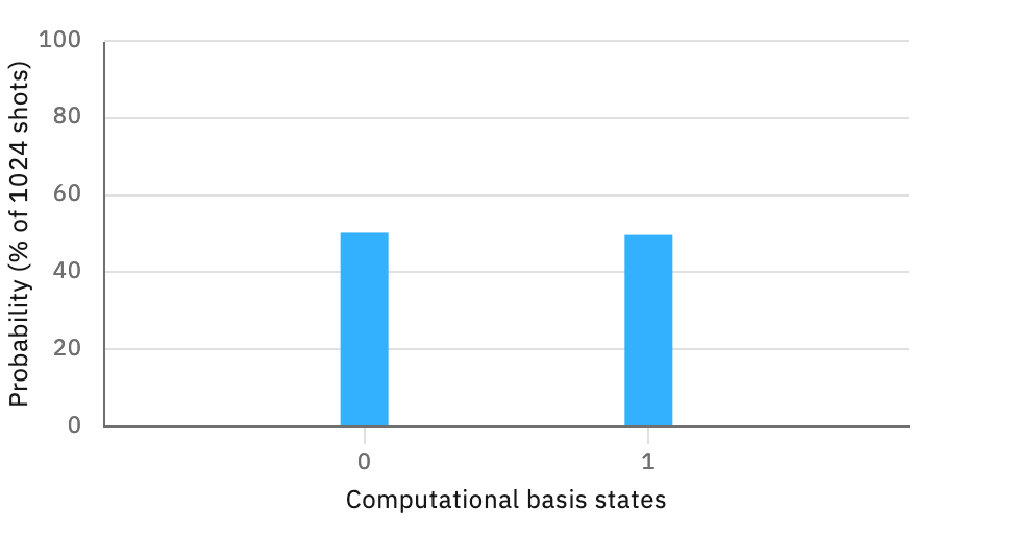
\includegraphics[width=0.95\textwidth]{./img/hgate_histogram.pdf}
        \caption{$H$ゲート回路の測定結果}
        \label{fig:hgate_result}
      \end{figure}
    \end{column}
  \end{columns}
\end{frame}

\begin{frame}
  \frametitle{1量子ビットのシミュレータ実験}

  \begin{columns}
    \begin{column}{0.4\textwidth}
      \begin{figure}
        \HGateFigure
      \end{figure}
    \end{column}
    \begin{column}{0.6\textwidth}
      \begin{itemize}
        \item $H$ゲートは$n$中心に$\pi$回転なので次のように2回やれば元の$\ket{0}$に戻る
        \begin{figure}
          \centering
          \scalebox{1.0}{
          \Qcircuit @C=1.0em @R=0.2em @!R {
            \lstick{\ket{0}} & \gate{H} & \gate{H} & \meter
          }}
        \end{figure}
        \begin{figure}
          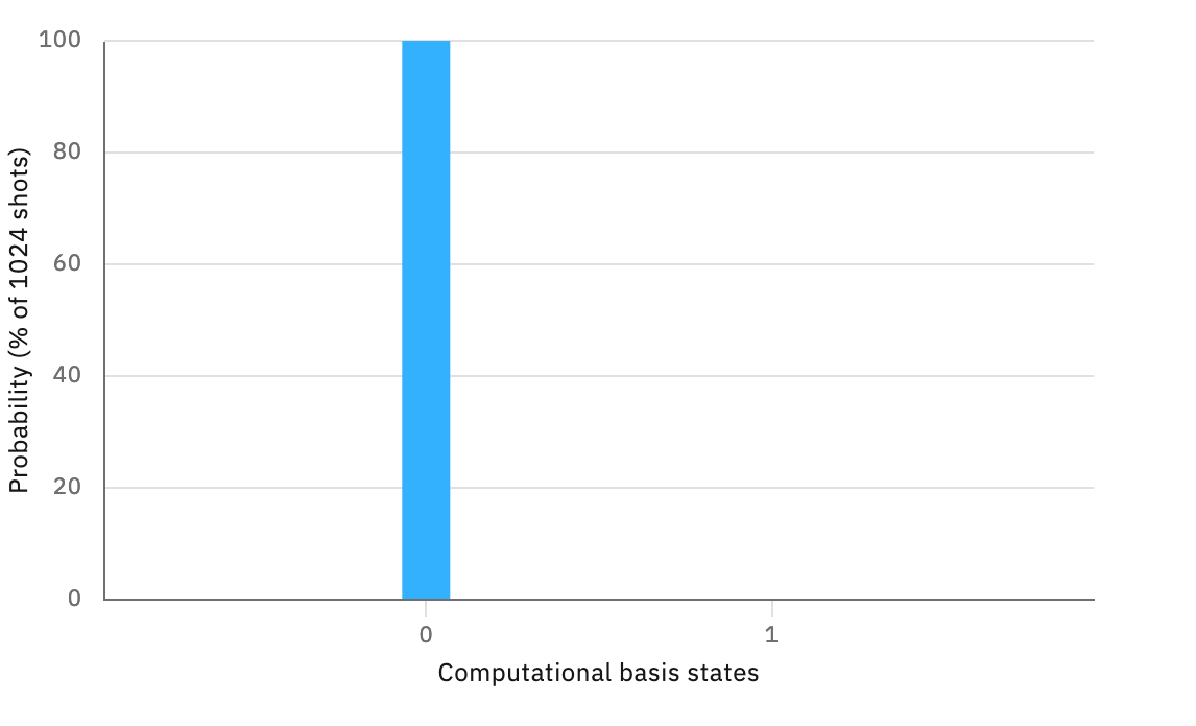
\includegraphics[width=0.7\textwidth]{./img/hgate_hgate_histogram.pdf}
        \end{figure}

        \item 同様に$H\ket{1} = \ket{-}$かつ$H\ket{-} = \ket{1}$となる
      \end{itemize}
    \end{column}
  \end{columns}
\end{frame}

\begin{frame}
  \frametitle{他の量子ゲート\ballcircle{1} --- $X$ゲート}

  \pause
  \begin{columns}
    \begin{column}{0.6\textwidth}
      \begin{itemize}
        \item<+-> $X$ゲートは図\ref{fig:x_gate_center}の$X$軸を中心に
        $\pi$回転させるゲート
        \begin{align*}
          X\ket{0} = \ket{1}, X\ket{1} = \ket{0}
        \end{align*}

        \item<+-> 古典コンピュータの\texttt{NOT}ゲートと似ている

        \item<+-> $X$軸上の$\ket{\pm}$に$X$ゲートを作用させても
        何も起きない
        \[
          X\ket{\pm} = \ket{\pm}
        \]
      \end{itemize}
    \end{column}
    \begin{column}{0.4\textwidth}
      \begin{figure}
        \begin{blochsphere}[radius=0.4\textwidth, tilt=15,rotation=-20,opacity=0.05]
          \drawBallGrid[style={opacity=0.1}]{40}{40}
        
          \drawAxis[style={cyan}]{0}{0}
          %\drawAxis[style={orange}]{90}{0}
          \drawCircle[style={red}]{0}{-90}
          %\drawAxis[style={orange}]{90}{90}
      
          \labelLatLon{n1}{0}{90};
          \labelLatLon{n2}{0}{-90};
          \draw[orange,->] (n2)--(n1);
          \drawSmallCircle[style={dashed, thick}]{90}{90}{0}
          
          \labelLatLon{x}{0}{90};
          \labelLatLon{y}{0}{0};
          \labelLatLon{z}{90}{90};
          \labelLatLon{down}{-90}{90};
          
          \node[above] at (z) {$\ket{0}$};
          \node[below] at (down) {$\ket{1}$};
          %\fill (z) ++(90:4ex) node {$Z$};
          %\node[above] at (y) {$Y$};
          \node[below left] at (x) {$\ket{+}$};
          \node[above right] at (n2) {$\ket{-}$};
          %\fill (x) ++(180:2em) node {$X$};
          \node[above] at (n1) {$X$};
        \end{blochsphere}
        \caption{$X$ゲートの回転中心}
        \label{fig:x_gate_center}
      \end{figure}
    \end{column}
  \end{columns}
\end{frame}

\begin{frame}
  \frametitle{他の量子ゲート\ballcircle{2} --- $Z$, $S$ゲート}

  \pause
  \begin{columns}
    \begin{column}{0.6\textwidth}
      \begin{itemize}
        \item<+-> $Z$ゲートは図\ref{fig:z_gate_center}の$Z$軸を中心に$\pi$回転させる

        \item<+-> $S$ゲートは$Z$軸を中心に$\frac{\pi}{2}$回転させる
        \begin{align*}
          Z\ket{+} = \ket{-}, Z\ket{-} = \ket{+}, SS\ket{+} = Z\ket{+} = \ket{-}
        \end{align*}

        \item<+-> $S\ket{\pm}$は$\left\{\ket{0}, \ket{1}\right\}$で次のように表現できる
        \begin{align*}
          S\ket{\pm} = \frac{1}{\sqrt{2}}\left(\ket{0} \pm \sqrt{-1}\ket{1}\right)
        \end{align*}

        \item<+-> $Z$軸上の$\ket{0}, \ket{1}$に$Z, S$ゲートを作用させても
        何も起きない
        \[
          Z\ket{0} = \ket{0}, S\ket{1} = \ket{1}
        \]
      \end{itemize}
    \end{column}
    \begin{column}{0.4\textwidth}
      \begin{figure}
        \begin{blochsphere}[radius=0.4\textwidth, tilt=15,rotation=-20,opacity=0.05]
          \drawBallGrid[style={opacity=0.1}]{40}{40}
        
          \drawAxis[style={blue}]{90}{0}
          \drawAxis[style={orange}]{90}{90}
      
          \labelLatLon{l}{0}{0};
          \labelLatLon{r}{180}{0};
          \labelLatLon{n1}{90}{0};
          \labelLatLon{n2}{-90}{0};
          \draw[cyan,->] (n2)--(n1);
          \drawSmallCircle[style={dashed, thick}]{0}{0}{0}
          
          \labelLatLon{x}{0}{90};
          \labelLatLon{y}{0}{0};
          \labelLatLon{z}{90}{90};
          \labelLatLon{down}{-90}{90};
          
          \labelLatLon{n3}{0}{-90};

          %\node[above] at (z) {$\ket{0}$};
          \node[below] at (down) {$\ket{1}$};
          %\fill (z) ++(90:4ex) node {$Z$};
          %\node[above] at (y) {$Y$};
          \node[below left] at (x) {$\ket{+}$};
          \node[above right] at (n3) {$\ket{-}$};
          \node[right] at (l) {$S\ket{+}$};
          \node[left] at (r) {$S\ket{-}$};
          %\fill (x) ++(180:2em) node {$X$};
          \node[above] at (n1) {$Z$};
        \end{blochsphere}
        \caption{$Z$, $S$ゲートの回転中心}
        \label{fig:z_gate_center}
      \end{figure}
    \end{column}
  \end{columns}
\end{frame}

\begin{frame}
  \frametitle{2量子ビットゲート}

  \begin{itemize}
    \item<+-> ここまでは次のような1量子ビットに対する量子ゲートを扱った
    \begin{itemize}
      \item $H$ゲート
      \item $X$ゲート
      \item $Z$ゲート
      \item $S$ゲート
    \end{itemize}

    \item<+-> 古典コンピュータの\texttt{NAND}ゲートのように、
    量子コンピュータにも2量子ビットを入力に持つゲートが存在する
  \end{itemize}
\end{frame}

\begin{frame}
  \frametitle{$CZ$ゲート}

  \pause
  \begin{itemize}
    \item $CZ$ゲートは2量子ビットを入力に持ち、
    \begin{enumerate}
      \item 1量子ビット目が$\ket{0}$であれば何もせず、
      \item 一方で1量子ビット目が$\ket{1}$であれば2量子ビット目に$Z$ゲートを作用させる
    \end{enumerate}
  \end{itemize}

  \pause
  \bobcallout{+}{1量子ビット目が$\ket{+}$だったら?}

  \pause
  \alicecallout{-}{%
    \begin{minipage}{0.8\textwidth}
      1量子ビット目を測定した結果、
      \begin{description}
        \item[$\ket{0}$が観測される] なにも起きない
        \item[$\ket{1}$が観測される] 2量子ビット目に$Z$ゲートが作用する
      \end{description}
    \end{minipage}
  }
\end{frame}

\begin{frame}
  \frametitle{$CZ$ゲート}

  \begin{columns}
    \begin{column}{0.5\textwidth}
      \begin{itemize}
        \item $CZ$ゲートを次のような量子回路\ref{fig:cz_gate}で確認してみる
      \end{itemize}
    \end{column}
    \begin{column}{0.47\textwidth}
      \begin{figure}
        \scalebox{1.0}{
        \Qcircuit @C=1.0em @R=0.2em @!R {
          \lstick{\ket{0}_1} & \gate{H} & \ctrl{1} & \meter \\
          \lstick{\ket{0}_2} & \gate{H\ballref{enum:cz_gate_1}} & \gate{Z\ballref{enum:cz_gate_2}} & \gate{H\ballref{enum:cz_gate_3}} & \meter
        }}
        \caption{$CZ$ゲートを用いた回路}
        \label{fig:cz_gate}
      \end{figure}
    \end{column}
  \end{columns}

  \pause
  \begin{itemize}
    \item<+-> 2量子ビット目の$\ket{0}_2$について考えると
    \begin{enumerate}
      \item $H$ゲートにより$\ket{+}$となる \label{enum:cz_gate_1}

      \item $CZ$ゲートによって、$Z$ゲートが作用しなければ$\ket{+}$のままであり、
      $Z$ゲートが作用すれば$\ket{-}$となる \label{enum:cz_gate_2}

      \item 最後に$H$ゲートを作用させるが、このとき
      $\ket{+}$であれば$H\ket{+} = \ket{0}$となり、
      一方で$\ket{-}$であれば$H\ket{-} = \ket{1}$となる \label{enum:cz_gate_3}
    \end{enumerate}

    \item<+-> 1量子ビット目は$\ket{+}$なので、$\ket{0}, \ket{1}$のどちらかになるかは確率$\frac{1}{2}$となる
  \end{itemize}
\end{frame}

\begin{frame}
  \frametitle{$CZ$ゲート}

  \begin{columns}
    \begin{column}{0.5\textwidth}
      \begin{figure}
        \scalebox{1.0}{
        \Qcircuit @C=1.0em @R=0.2em @!R {
          \lstick{\ket{0}_1} & \gate{H} & \ctrl{1} & \meter \\
          \lstick{\ket{0}_2} & \gate{H} & \gate{Z} & \gate{H} & \meter
        }}
      \end{figure}
    \end{column}
    \begin{column}{0.5\textwidth}
      \bobcallout{-}{\ce{:point_left:}つまりまとめると……}
    \end{column}
  \end{columns}

  \pause
  \begin{itemize}
    \item 確率$\frac{1}{2}$で1量子ビット目の測定結果が$\ket{0}$なら2量子ビット目も$\ket{0}$
    \item 確率$\frac{1}{2}$で1量子ビット目の測定結果が$\ket{1}$なら2量子ビット目も$\ket{1}$
  \end{itemize}

  \pause
  \alicecallout{-}{シミュレーターでやってみる!}
\end{frame}

\begin{frame}
  \frametitle{$CZ$ゲートのシミュレーション結果}

  \begin{center}
    \begin{figure}
      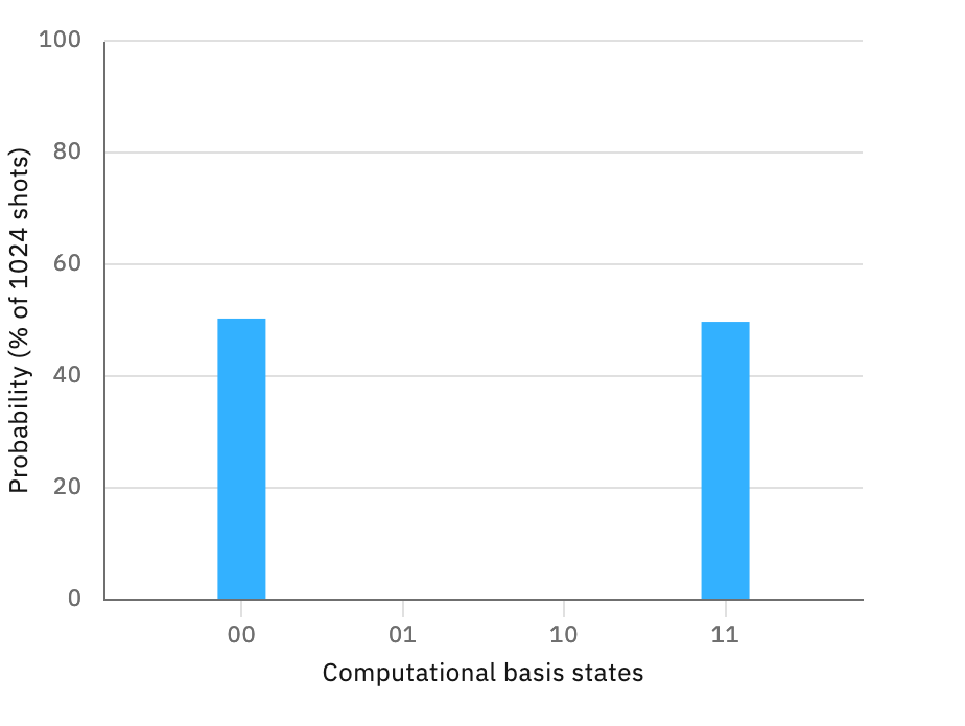
\includegraphics[width=0.45\textwidth]{./img/cz_gate_histogram.pdf}
      \caption{%
        $CZ$ゲートを使った回路のシミュレーション結果%
        \footnote{図の最下位ビットが1量子ビット目、最上位ビットが2量子ビット目となる。}%
      }
    \end{figure}
  \end{center}

  \pause
  \begin{itemize}
    \item このように\ce{:point_up:}シミュレーション結果は$\ket{00}$か$\ket{11}$が$\frac{1}{2}$となる\ce{:person_gesturing_ok:}
  \end{itemize}
\end{frame}

\section{量子ゲートテレポーテーション}

\begin{frame}
  \frametitle{$CZ$ゲート後の量子操作と測定}

  \pause
  \begin{itemize}
    \item<+-> 2つの量子ビットが$\ket{+}$のとき、$CZ$ゲートを用いた
    図\ref{fig:teleportation_circuit}の回路を考える
    \begin{enumerate}
      \item $Z$軸の回転ゲートを作用させ \label{enum:teleportation_1}
      \item $H$ゲートを作用させ \label{enum:teleportation_2}
      \item 測定を行う \label{enum:teleportation_3}
    \end{enumerate}

    \begin{columns}
      \begin{column}{0.6\textwidth}
        \begin{figure}
          \centering
          \scalebox{1.0}{
          \Qcircuit @C=1.0em @R=0.2em @!R {
            \lstick{\ket{0}_1} & \gate{H} & \ctrl{1} & \gate{Z\ballref{enum:teleportation_1}} & \gate{H\ballref{enum:teleportation_2}} & \meter & \ballref{enum:teleportation_3} \\
            \lstick{\ket{0}_2} & \gate{H} & \gate{Z} & \qw & \meter
          }}
          \caption{$CZ$ゲートの後で$Z, H$ゲートを作用させ測定}
          \label{fig:teleportation_circuit}
        \end{figure}

        \uncover<+(1)->{%
          \bobcallout{-}{%
            1量子ビット目は常に$\ket{1}$では?\ce{:thinking:}\\
            $HZH\ket{0}_1 = HZ\ket{+}_1 = H\ket{-}_1 = \ket{1}_1$
          }
        }
      \end{column}
      \begin{column}{0.4\textwidth}
        \uncover<+(-1)->{%
          \begin{figure}
            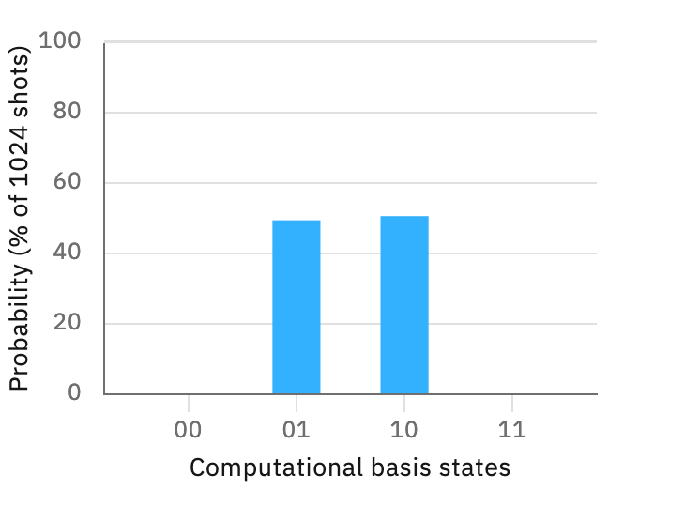
\includegraphics[width=0.8\textwidth]{./img/cz_teleportation_histogram.pdf}
            \caption{回路\ref{fig:teleportation_circuit}のシミュレーション結果}
          \end{figure}
        }
      \end{column}
    \end{columns}
  \end{itemize}
\end{frame}

\begin{frame}
  \frametitle{量子ゲートテレポーテーション}

  \begin{columns}
    \begin{column}{0.6\textwidth}
      \begin{figure}
        \centering
        \scalebox{1.0}{
        \Qcircuit @C=1.0em @R=0.4em @!R {
          \lstick{\ket{0}_1} & \gate{H} & \ctrl{1} & \gate{Z\ballref{enum:teleportation_1}} & \gate{H\ballref{enum:teleportation_2}} & \meter & \ballref{enum:teleportation_3}  \gategroup{1}{5}{1}{4}{.6em}{--} \\
          \lstick{\ket{0}_2} & \gate{H} & \gate{Z} & \qw & \meter
        }}
      \end{figure}
    \end{column}
    \begin{column}{0.4\textwidth}
      \begin{figure}
        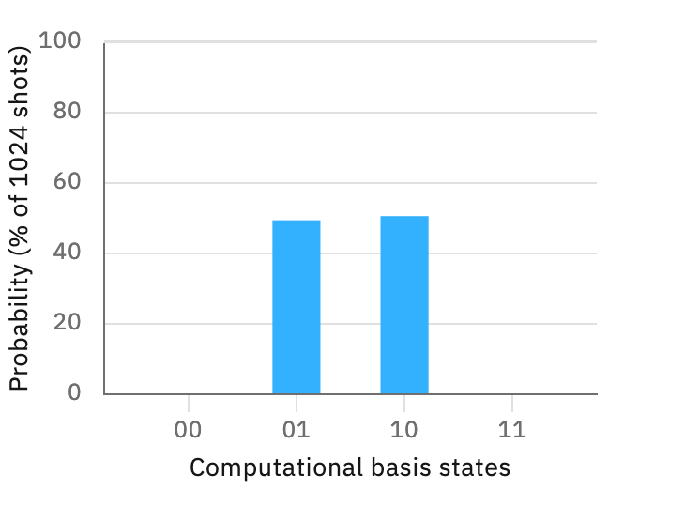
\includegraphics[width=0.6\textwidth]{./img/cz_teleportation_histogram.pdf}
      \end{figure}
    \end{column}
  \end{columns}

  \begin{itemize}
    \item 図\ref{fig:teleportation_0},\ref{fig:teleportation_1}のように
    $Z,H$ゲートが2量子ビット目へ\textbf{テレポーテーション}する
    \begin{itemize}
      \item 1量子ビット目の測定結果に応じて$X$ゲートの有無の差がある
    \end{itemize}
  \end{itemize}

  \begin{columns}
    \begin{column}{0.5\textwidth}
      \begin{figure}
        \scalebox{1.0}{
        \Qcircuit @C=1.0em @R=0.2em @!R {
          \lstick{\ket{0}_2} & \gate{H} & \gate{Z\ballref{enum:teleportation_1}} & \gate{H\ballref{enum:teleportation_2}} & \meter
        }}
        \caption{1量子ビット目の測定結果が$0$}
        \label{fig:teleportation_0}
      \end{figure}
    \end{column}
    \begin{column}{0.5\textwidth}
      \begin{figure}
        \scalebox{1.0}{
        \Qcircuit @C=1.0em @R=0.2em @!R {
          \lstick{\ket{0}_2} & \gate{H} & \gate{Z\ballref{enum:teleportation_1}} & \gate{H\ballref{enum:teleportation_2}} & \gate{X} & \meter
        }}
        \caption{1量子ビット目の測定結果が$1$}
        \label{fig:teleportation_1}
      \end{figure}
    \end{column}
  \end{columns}
  
  \pause
  \begin{itemize}
    \item $Z$軸上の回転ゲートである$S$ゲートもテレポーテーションできる
  \end{itemize}
\end{frame}

\begin{frame}
  \frametitle{量子ゲートテレポーテーション}

  \begin{itemize}
    \item テレポーテーションなので1量子ビット目から$Z, H$ゲートが\textbf{消える}
    \begin{itemize}
      \item テレポーテーションであってコピーではない
    \end{itemize}
  \end{itemize}

  \begin{columns}
    \begin{column}{0.5\textwidth}
      \begin{figure}
        \scalebox{1.0}{
        \Qcircuit @C=1.0em @R=0.2em @!R {
          \lstick{\ket{0}_1} & \gate{H} & \ctrl{1} & \gate{H} & \meter \\
          \lstick{\ket{0}_2} & \gate{H} & \gate{Z} & \meter
        }}
        \caption{$H$ゲートだけのテレポーテーション}
        \label{fig:h_gate_teleportation}
      \end{figure}
    \end{column}
    \begin{column}{0.5\textwidth}
      \begin{figure}
        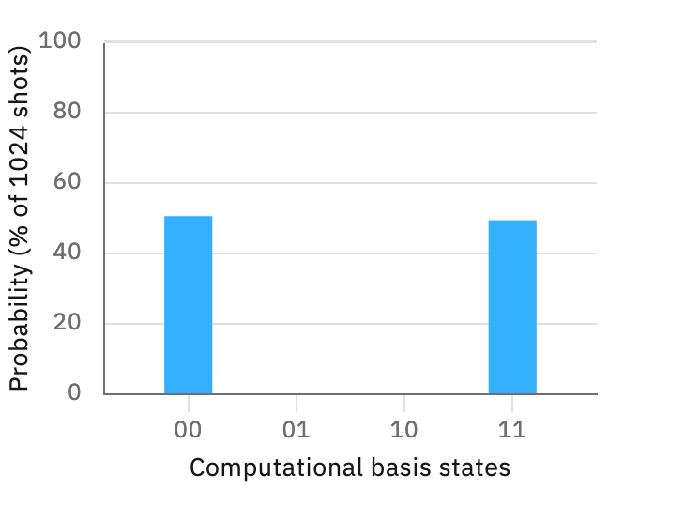
\includegraphics[width=0.5\textwidth]{./img/h_gate_teleportation.pdf}
        \caption{回路\ref{fig:h_gate_teleportation}のシミュレーション結果}
        \label{fig:h_gate_teleportation_histogram}
      \end{figure}
    \end{column}
  \end{columns}

  \pause
  \begin{itemize}
    \item<+-> 1量子ビット目は$H$ゲートが2回作用しているので、$CZ$ゲートがなければキャンセルして常に$\ket{0}$となる

    \item<+-> しかし図\ref{fig:h_gate_teleportation_histogram}では
    1量子ビット目が$\ket{0},\ket{1}$のランダムとなっている
  \end{itemize}
\end{frame}

\begin{frame}
  \frametitle{量子ゲートテレポーテーション}

  \alicecallout{-}{$CZ$ゲートで$Z, S, H$ゲートをテレポーテーションできる!}    

  \pause
  \bobcallout{+}{そんなことある?\ce{:thinking:}}

  \pause
  \alicecallout{-}{量子コンピュータ(= 宇宙?)はこういうもの!}
\end{frame}

\section{Quantum Covert Lottery}

\begin{frame}
  \frametitle{Quantum Covert Lottery}

  \begin{columns}
    \begin{column}{0.55\textwidth}
      \begin{minipage}[t][.6\textheight][t]{\textwidth}
        \tableofcontents[currentsection]
      \end{minipage}
    \end{column}
    \begin{column}{0.45\textwidth}
      \pause
      \begin{itemize}
        \item<+-> もっと色々な量子ゲートがある

        \item<+-> 量子コンピュータ上のCovert Lotteryの説明はここまでの量子ゲートでOK\ce{:person_gesturing_ok:}
        \begin{itemize}
          \item $X, S, Z, H$ゲート
          \item $CZ$ゲート
        \end{itemize}
        
        \item<+-> シュレディンガーの猫と量子ゲートテレポーテーションで``Quantum Covert Lottery''を作っていく
      \end{itemize}
    \end{column}
  \end{columns}
\end{frame}

\begin{frame}
  \frametitle{プロトコル}

  \pause
  \begin{enumerate}
    \item<+-> アリスは表\ref{tbl:covert_meaning_2}にしたがって希望$a \in \{0, 1\}$と、
    乱数$x \in \{0, 1\}$を生成する

    \item<+-> アリスは次のような回路\ref{fig:alice_circuit}で表現される3量子ビットを用意する
    \begin{itemize}
      \item $a = 1$であれば、1量子ビット目に$S$ゲートを作用させる
      \item $x = 1$であれば、3量子ビット目に$Z$ゲートを作用させる
    \end{itemize}
    \label{enum:alice_s_z_gate}

    \item<+-> 3量子ビットを量子通信回線でボブへ送信する
  \end{enumerate}

  \begin{columns}
    \begin{column}{0.5\textwidth}
      \uncover<+(-2)->{%
        \begin{figure}
          \centering
          \scalebox{0.8}{
          \Qcircuit @C=1.0em @R=0.2em @!R {
            \lstick{a}         & \cw      & \cw             & \control\cw \\
            \lstick{\ket{0}_1} & \gate{H} & \ctrl{1}        & \gate{S\ballref{enum:alice_s_z_gate}}\cwx & \qw      & \qw\\
            \lstick{\ket{0}_2} & \gate{H} & \gate{Z}        & \ctrl{1}     & \qw      & \qw\\
            \lstick{\ket{0}_3} & \gate{H} & \gate{Z\ballref{enum:alice_s_z_gate}}\cwx[1] & \gate{Z}     & \gate{H} & \qw \\
            \lstick{x}         & \cw      & \control\cw
          }}
          \caption{アリスの用意する3量子ビット}
          \label{fig:alice_circuit}
        \end{figure}
      }
    \end{column}
    \begin{column}{0.5\textwidth}
      \uncover<+(-4)->{%
        \begin{table}[h]
          \caption{希望とビットの対応}
          \begin{tabularx}{0.7\textwidth}{@{}| Y | Y |@{}}
            \hline
            希望 & 意味 \\ \hline
            $0$ & ボブの奢り \\ \hline
            $1$ & 割り勘 \\ \hline
          \end{tabularx}
          \label{tbl:covert_meaning_2}
        \end{table}
      }
    \end{column}
  \end{columns}
\end{frame}

\begin{frame}
  \frametitle{プロトコル}

  \begin{enumerate}
    \setcounter{enumi}{3}

    \item<+-> ボブはアリスから3量子ビットを受けとる
    
    \item<+-> ボブは希望$b \in \{0, 1\}$を選び図\ref{fig:bob_circuit}のような量子操作を行う
    \begin{itemize}
      \item $b = 1$であれば1量子ビット目に$S$ゲートを作用させる
    \end{itemize}
    \label{enum:bob_s_gate}

    \item<+-> ボブは1量子ビット目に$H$ゲートを作用させる
    \label{enum:bob_h_gate}
  \end{enumerate}

  \uncover<2->{
    \begin{figure}
      \scalebox{1.0}{
        \Qcircuit @C=1.0em @R=0.2em @!R {
          \lstick{b}         & \cw      & \cw       & \cw        & \control\cw \\
          \lstick{\ket{0}_1} & \gate{H} & \ctrl{1}  & \gate{S^?} & \gate{S\ballref{enum:bob_s_gate}}\cwx & \gate{H\ballref{enum:bob_h_gate}} & \qw \\%& \control \cw \\
          \lstick{\ket{0}_2} & \gate{H} & \gate{Z}  & \ctrl{1}   & \qw          & \qw    \\%& \gate{X}\cwx & \meter \\
          \lstick{\ket{0}_3} & \gate{H} & \gate{Z^?} & \gate{Z}  & \gate{H}     & \qw    %& \gate{X}\cwx
      }}%
      \caption{ボブが行う量子操作}
      \label{fig:bob_circuit}
    \end{figure}
  }
\end{frame}

\begin{frame}
  \frametitle{プロトコル}

  \begin{columns}
    \begin{column}{0.5\textwidth}
      \bobcallout{-}{これどういうこと?}    
    \end{column}
    \begin{column}{0.5\textwidth}
      \pause
      \alicecallout{+}{1量子ビット目だけ整理してみる}
    \end{column}
  \end{columns}

  \begin{itemize}
    \item<+-> 1量子ビット目とアリス・ボブの希望$a,b$に注目すると図\ref{fig:1st_qubit}の回路になる
    \begin{figure}
      \centering
      \scalebox{1.0}{
      \Qcircuit @C=1.0em @R=0.2em @!R {
        \lstick{a}         & \cw      & \cw          & \control\cw \\
        \lstick{\ket{0}_1} & \gate{H} & \ctrl{1}     & \gate{S}\cwx & \gate{S}\cwx[1] & \gate{H} & \meter \\
        \lstick{b}         & \cw      & \cw          & \cw          & \control\cw
      }}
      \caption{1量子ビット目とアリス・ボブの希望$a, b$}
      \label{fig:1st_qubit}
    \end{figure}

    \item<+-> これをアリス・ボブの希望$a, b$で場合わけして考える
  \end{itemize}
\end{frame}

\begin{frame}
  \frametitle{ケーススタディ\ballcircle{1} --- アリス・ボブの希望が一致}

  \begin{itemize}
    \item アリス・ボブの希望が一致するときは$a = b$なので次の2つになる
  \end{itemize}

  \begin{columns}
    \begin{column}{0.5\textwidth}
      \begin{figure}
        \scalebox{1.0}{
        \Qcircuit @C=1.0em @R=0.2em @!R {
          \lstick{\ket{0}_1} & \gate{H} & \ctrl{1}    & \gate{H} & \meter \\
                              &          &
        }}
        \caption{両者がボブの奢り($0$)で一致}
        \label{fig:a_equal_0}
      \end{figure}
    \end{column}
    \begin{column}{0.5\textwidth}
      \begin{figure}
        \scalebox{1.0}{
        \Qcircuit @C=1.0em @R=0.2em @!R {
          \lstick{\ket{0}_1} & \gate{H} & \ctrl{1} & \gate{S} & \gate{S} & \gate{H} & \meter \\
                              &          &
        }}
        \caption{両者が割り勘($1$)で一致}
        \label{fig:a_equal_1}
      \end{figure}
    \end{column}
  \end{columns}

  \pause
  \begin{itemize}
    \item $SS = Z$により、2量子ビット目へのテレポーテーション内容は次のようになる
    \begin{description}
      \item[$a = b = 0$] $H$ゲート(+ $X$ゲート)
      \item[$a = b = 1$] $H$ゲートと$Z$ゲート(+ $X$ゲート)
    \end{description}
  \end{itemize}

  \pause
  \alicecallout{-}{$S$ゲートがテレポーテーションしないのがポイント!}  
\end{frame}

\begin{frame}
  \frametitle{ケーススタディ\ballcircle{2} --- アリス・ボブの希望が不一致}

  \pause
  \begin{itemize}
    \item<+-> 一方で、アリス・ボブの希望が一致しない場合$a \ne b$なので次のようになる
    \begin{figure}
      \scalebox{1.0}{
      \Qcircuit @C=1.0em @R=0.2em @!R {
        \lstick{\ket{0}_1} & \gate{H} & \ctrl{1}    & \gate{S}  & \gate{H} & \meter \\
                           &          & 
      }}
      \caption{アリスは割り勘・ボブは奢り、またはアリスは奢り・ボブは割り勘}
      \label{fig:a_eq_1_b_eq_0}
    \end{figure}
  
    \item<+-> いずれも$S$ゲートと$H$ゲートが2量子ビット目へテレポーテーションする
  \end{itemize}

  \uncover<+->{%
    \bobcallout{+}{$S$ゲートが2量子ビット目へテレポーテーションされる!}
  }
\end{frame}

\begin{frame}
  \frametitle{プロトコル}

  \begin{enumerate}
    \setcounter{enumi}{6}

    \item<+-> ボブは1量子ビット目の測定を行い測定結果を$c_1$とする
    \begin{figure}
      \scalebox{1.0}{
        \Qcircuit @C=1.0em @R=0.2em @!R {
          \lstick{\ket{0}_1} & \gate{H} & \ctrl{1}  & \gate{S^?} & \gate{S^?} & \gate{H} & \meter & \rstick{\rightarrow c_1} \\
                             &          & 
      }}%
    \end{figure}

    \item<+-> ボブは$c_1 = 1$なら次のように$X$ゲートを2, 3量子ビット目に作用させる
    \begin{figure}
      \scalebox{1.0}{
        \Qcircuit @C=1.0em @R=0.2em @!R {
                            &          &  \\
          \lstick{c_1}       & \cw      & \cw               & \cw       & \cw      & \control\cw \\
          \lstick{\ket{0}_2} & \gate{H} & \gate{Z}\qwx[-2]  & \ctrl{1}  & \qw      & \gate{X}\cwx & \qw \\
          \lstick{\ket{0}_3} & \gate{H} & \gate{Z^?}        & \gate{Z}  & \gate{H} & \gate{X}\cwx & \qw
        }}
    \end{figure}
  \end{enumerate}

  \uncover<+->{%
    \bobcallout{+}{量子ゲートテレポーテーションで偶発的に生じる$X$ゲートをキャンセル!}
  }
\end{frame}

\begin{frame}
  \frametitle{プロトコル}

  \begin{enumerate}
    \setcounter{enumi}{8}

    \item<+-> ボブは2量子ビット目の測定を行い結果を$c_2$とする
    \begin{figure}
      \scalebox{1.0}{
        \Qcircuit @C=1.0em @R=0.2em @!R {
                             &          &                   & \\
          \lstick{\ket{0}_2} & \gate{H} & \gate{Z}\qwx[-1]  & \ctrl{1}  & \meter & \rstick{\rightarrow c_2}\\
                             &          &                   &
        }}
    \end{figure}
    \label{enum:bob_measure_2nd_qubit}
    
    \item<+-> プロトコルの結果として$c_2$をアリスへ共有する
  \end{enumerate}

  \uncover<+->{%
    \alicecallout{-}{2, 3量子ビット目は希望$a, b$で場合わけ}
  }
\end{frame}

\begin{frame}
  \frametitle{\ballcircle{i} $a = b = 0$のとき}

  \begin{figure}
    \scalebox{1.0}{
      \Qcircuit @C=1.0em @R=0.2em @!R {
        \lstick{\ket{0}_2} & \gate{H} & \gate{H}   & \ctrl{1}  & \meter   & \rstick{\rightarrow c_2}\\
        \lstick{\ket{0}_3} & \gate{H} & \gate{Z^?} & \gate{Z}  & \gate{H} & \qw 
      }}
  \end{figure}

  \begin{itemize}
    \item<+-> $H$ゲートの相殺により2量子ビット目は$\ket{0}$に確定し$c_2 = 0$となる
    
    \item<+-> アリス・ボブの両方が「ボブの奢り」である$0$を希望しているため、
    プロトコルの結果として$0$となりOK\ce{:person_gesturing_ok:}
  \end{itemize}
\end{frame}

\begin{frame}
  \frametitle{\ballcircle{ii} $a = b = 1$のとき}

  \begin{figure}
    \scalebox{1.0}{
      \Qcircuit @C=1.0em @R=0.2em @!R {
        \lstick{\ket{0}_2} & \gate{H} & \gate{Z}   & \gate{H} & \ctrl{1}  & \meter   & \rstick{\rightarrow c_2} \\
        \lstick{\ket{0}_3} & \gate{H} & \gate{Z^?} & \qw      & \gate{Z}  & \gate{H} & \qw
      }}
  \end{figure}

  \begin{itemize}
    \item<+-> $H,Z,H$ゲート操作で2量子ビット目は$\ket{1}$に確定し$c_2 = 1$となる
    \[
      HZH\ket{0}_2 = HZ\ket{+}_2 = H\ket{-}_2 = \ket{1}_2
    \]

    \item<+-> アリス・ボブの両方が「割り勘」である$1$を希望しているため、
    プロトコルの結果として$1$となりOK\ce{:person_gesturing_ok:}
  \end{itemize}
\end{frame}

\begin{frame}
  \frametitle{\ballcircle{iii} $a \ne b$のとき}

  \begin{figure}
    \scalebox{1.0}{
      \Qcircuit @C=1.0em @R=0.2em @!R {
        \lstick{\ket{0}_2} & \gate{H} & \gate{S}   & \gate{H} & \ctrl{1} & \meter   & \rstick{\rightarrow c_2} \\
        \lstick{\ket{0}_3} & \gate{H} & \gate{Z^?} & \qw      & \gate{Z} & \gate{H} & \qw 
      }}
  \end{figure}

  \begin{itemize}
    \item<+-> $H,S,H$ゲート操作で2量子ビット目は$S\ket{-}$となる
    \begin{itemize}
      \item $S\ket{-}$はブロッホ球の赤道上なので、測定結果は$\ket{0}, \ket{1}$が$\frac{1}{2}$となる
    \end{itemize}

    \item<+-> アリス・ボブの希望が割れた場合は結果は$0, 1$の50\%ランダムとなりOK\ce{:person_gesturing_ok:}
  \end{itemize}
\end{frame}

\begin{frame}
  \frametitle{プロトコル}

  \begin{columns}
    \begin{column}{0.5\textwidth}
      \pause
      \bobcallout{-}{3量子ビット目は?}  
    \end{column}
    \begin{column}{0.5\textwidth}
      \pause
      \alicecallout{+}{ボブの不正検知!}
    \end{column}
  \end{columns}

  \pause
  \begin{enumerate}
    \setcounter{enumi}{10}

    \item<+-> ボブは3量子ビット目を測定し$c_3$としアリスへ送信する
    \begin{figure}
      \scalebox{1.0}{
        \Qcircuit @C=1.0em @R=0.2em @!R {
                             &          &            &   \\
          \lstick{\ket{0}_3} & \gate{H} & \gate{Z^?} & \gate{Z}\qwx[-1] & \gate{H} & \meter & \rstick{\rightarrow c_3} 
        }}
    \end{figure}

    \item<+-> アリスはボブから$c_2, c_3$を受け取り、式\ref{eq:alice_check}を確認する
    \begin{align}
      c_2\; \mathtt{XOR}\; x \stackrel{?}{=} c_3 \label{eq:alice_check}
    \end{align}
    \begin{itemize}
      \item 式\ref{eq:alice_check}が等しくなければプロトコルを中止する
    \end{itemize}
  \end{enumerate}
\end{frame}

\begin{frame}
  \frametitle{ボブの不正検知}

  \pause
  \begin{itemize}
    \item<+-> 二人の希望が衝突した場合、
    ボブは\ballref{enum:bob_measure_2nd_qubit}で都合がいい$c_2$が観測されたと偽ることができる\ce{:smiling_imp:}

    \item<+-> 式\ref{eq:alice_check}により、アリスは確率$\frac{1}{2}$でボブの不正を検知できる

    \item<+-> 検証用の量子ビットを$n$ qubit用意すれば$\frac{1}{2^n}$でボブの不正を困難にできる
    \begin{itemize}
      \item 図\ref{fig:bob_cheat_detection}の回路ではボブは$x_1, x_2, x_3$の3bitを
      全てあてなければ不正に成功しない
    \end{itemize}
  \end{itemize}

  \uncover<.->{%
    \begin{figure}
      \scalebox{0.8}{
        \Qcircuit @C=1.0em @R=0.2em @!R {
                            &          &                &                  &                  &          &     &  \\ 
          \lstick{\ket{0}_2} & \gate{H} & \qw            & \gate{Z}\qwx[-1] & \ctrl{1}         & \qw      & \qw & \gate{X}\cwx[-1] & \meter \\
          \lstick{\ket{0}_3} & \gate{H} & \gate{Z^{x_1}} & \qw              & \gate{Z}\ctrl{1} & \gate{H} & \qw & \gate{X}\cwx[-1] & \meter & \rstick{\rightarrow c_3}\\
          \lstick{\ket{0}_4} & \gate{H} & \gate{Z^{x_2}} & \qw              & \gate{Z}\ctrl{1} & \gate{H} & \qw & \gate{X}\cwx[-1] & \meter & \rstick{\rightarrow c_4}\\
          \lstick{\ket{0}_5} & \gate{H} & \gate{Z^{x_3}} & \qw              & \gate{Z}         & \gate{H} & \qw & \gate{X}\cwx[-1] & \meter & \rstick{\rightarrow c_5}\\
        }}
      \caption{ボブの不正対策を増やした回路}
      \label{fig:bob_cheat_detection}
    \end{figure}
  }
\end{frame}

% \begin{frame}
%   \begin{figure}
%     \centering
%     \scalebox{1.0}{
%     \Qcircuit @C=1.0em @R=0.2em @!R {
%       \lstick{\ket{q_0}} & \gate{H} & \gate{S} & \ctrl{1} & \gate{S} & \gate{H} & \meter  & \control \cw \\
%       \lstick{\ket{q_1}} & \gate{H} & \qw      & \gate{Z} & \ctrl{1} & \qw      & \qw     & \gate{X}\cwx & \meter & \rstick{\cdots\; c_1} \\
%       \lstick{\ket{q_2}} & \gate{H} & \qw      & \qw      & \gate{Z} & \gate{H} & \qw     & \gate{X}\cwx & \meter & \rstick{\cdots\; c_2}
%     }}
%     \caption{量子Covert Lotteryの回路}
%   \end{figure}
% \end{frame}

\section{まとめ}

\begin{frame}
  \frametitle{まとめ}

  \pause
  \begin{itemize}
    \item<+-> 量子コンピュータを用いた``Quantum Covert Lottery''で
    奢り・割り勘問題に決着をつけられるかもしれない
    \begin{itemize} 
      \item すでにインターネットで公開しているプロトコル\cite{quantum_covert_lottery}は
      ボブの不正対策がない\ce{:innocent:}
    \end{itemize}

    \item<+-> ボブは困難とはいえ不正ができるが、アリスの不正が今のところない。
    \begin{itemize} 
      \item アリスもボブと全く同じ困難性で不正ができるようにしたい
    \end{itemize}

    \item<+-> 今回は2人だったが、これを多人数拡張すると別のゲームに使えるかも\ce{:thinking_face:}
    \begin{itemize}
      \item 量子版の多人数拡張はまだできてない……\ce{:innocent:}
    \end{itemize}

    \item<+-> 量子コンピュータには高速な素因数分解といったアルゴリズム高速化以外にも
    色々な応用の可能性があると思う
    \begin{itemize}
      \item シュレディンガーの猫や量子ゲートテレポーテーションはそれだけで夢がある
    \end{itemize}
  \end{itemize}
\end{frame}

\section*{参考文献}
\begin{frame}[allowframebreaks]
  \frametitle{参考文献}
  %\nocite{*}
  \bibliographystyle{junsrt_url}
  \bibliography{ref}
\end{frame}

\begin{frame}
  \centering
  {\Huge Thank you for the attention!}
\end{frame}

\end{document}
